\documentclass[12pt,a4paper,titlepage]{article}
\usepackage[a4paper,left=25mm,right=15mm,top=20mm,bottom=20mm]{geometry}
\usepackage[utf8]{inputenc}
\usepackage[L7x]{fontenc}
\usepackage[lithuanian]{babel}
\usepackage{amsmath}
\usepackage{amsfonts}
\usepackage{amssymb}
\usepackage{setspace}
\usepackage{mathptmx}
\usepackage{graphicx}
\usepackage{float}
\onehalfspacing
\usepackage[backend=biber, style=apa, url=false, sorting=nyt]{biblatex}
\addbibresource{references.bib}
\title{Gyventojų pajamų nelygybė Lietuvoje nuo 2008 m.}
\author{Armintė Globytė}
\date{2019 m.}
\begin{document}
\maketitle
\newpage
\setcounter{tocdepth}{3}
\setcounter{secnumdepth}{3}
\tableofcontents
\newpage
\section{Įvadas}
Pajamų nelygybė – reiškinys, pastaruoju metu sulaukiantis vis daugiau dėmesio. Girdime politikų kalbas, skaitome straipsnius, kuriuose užsimenama apie gyventojų sluoksniavimąsi, socialinę atskirtį, nelygybę. Pasaulyje pradeda plisti nuomonė, kad ekonominius šalies pasiekimus ir gyventojų socialinę gerovę atspindi ne tik BVP rodiklis, bet ir BVP perskirstymas. Pagal 2019 metų Europos Komisijos ataskaitą, Lietuvos ekonomika išlaiko tvirtą augimo pagreitį, tačiau pajamų nelygybė tebėra viena didžiausių Europos Sąjungoje. Europos socialinių teisių ramstį pagrindžiančios socialinių rodiklių suvestinės duomenimis, pajamų nelygybės lygis Lietuvoje yra kritinis. Lietuva nedaro pakankamos pažangos, kad pajamų nelygybė būtų sumažinta, mokesčių ir socialinių išmokų sistemos pajėgumas yra silpnas, Lietuvos išlaidos socialinei apsaugai yra mažos, o socialinių pervedimų poveikis skurdo mažinimui yra nedidelis. Pajamų nelygybę iš esmės lemia palyginti stiprus didžiausias pajamas gaunančių asmenų pajamų augimas. Privačiajame sektoriuje ribotas darbdavių ir profesinių sąjungų socialinis dialogas silpnina mažas pajamas gaunančių asmenų poziciją. 
\subsection{Pajamų nelygybės samprata}
Trumpai tariant, pajamų nelygybė – tai pajamų skirtumai tarp individų ekonomikoje. (\cite{skuvciene2008pajamku}) Nelygybė matuoja santykius tarp gyventojų dalies ir pajamų (išlaidų), kurias patiria ta gyventojų dalis. Statistiškai galima apibrėžti nelygybės ribas. Maksimali nelygybė būtų tuo atveju, jeigu vienas asmuo patirtų visas išlaidas. Minimali nelygybė būtų tada, jeigu visi gyventojai pasidalytų po vienodą išlaidų dalį.(\cite{vciulevivcius2008lietuvos}) Nelygybė dažnai tiriama kaip platesnė skurdo ir socialinės gerovės analizės dalis, tačiau šios trys sąvokos skiriasi. Nelygybė yra platesnė sąvoka nei skurdas, nes ji yra apima visą žmonių pasiskirstymą, o ne tik tą dalį asmenų ar namų ūkių, kurie yra žemiau tam tikros skurdo ribos. Norint suvokti ir įvertinti nelygybę, reikia įsidėmėti, kad pajamos, kurias gaunas viršuje ir viduryje pagal pasiskirstymą esantys žmonės ar namų ūkiai yra lygiai tokios pat svarbios kaip ir tų žmonių, kurie yra apačioje. Nelygybė taip pat yra daug siauresnė sąvoka nei socialinė gerovė. Nors abu jie užfiksuoja visą tam tikro rodiklio pasiskirstymą, nelygybė nepriklauso nuo pasiskirstymo vidurkio, o glaudžiai susijusi tik su paiskirstymo dispersija. Tačiau šios trys sąvokos yra giminingos ir kartais naudojamos kaip sudėtiniai matai skaičiavimuose. (\cite{litchfield1999inequality}) 
\subsection{Kodėl svarbu kalbėti apie pajamų nelygybę?}
Pagal atliktus tyrimus, pajamų nelygybė daro įtaką sveikatai, išsilavinimui, skatina nusikalstamumą, didėja mirtingumo rodikliai. Skurstančių žmonių galimybės, palyginti su didžiausias pajamas gaunančių gyventojų galimybėmis, yra labai apribotos. Su augančia pajamų nelygybe siejami sunkumai jaunoms šeimoms įsigyti ar išsinuomoti butą, padidėjęs būsto perkrovimas, neadekvačios būsto sąlygos nepasiturintiems vaikams. Didesnės pajamos užtikrina didesnes galimybes įsigyti prekes ir paslaugas, kurios palaiko sveikatą: geresnį maitinimą, geros kokybės sveikatos paslaugas,o nepasiturintys žmonės turi didesnę sergamumo riziką, turi rinktis prastesnės kokybės švietimo įstaigas.(\cite{skuvciene2008pajamku}) Šios neigiamos pajamų nelygybės pasėkmės yra labai svarbios ir parodo, kad pajamų nelygybės problemai turėtų būti skiriama ypač daug dėmesio. 
\section{Pajamų nelygybės matavimai}
\subsection{Džini koeficientas}
Džini (Gini) koeficientas yra pajamų pasiskirstymo nelygybės šalyje
rodiklis. Jis apskaičiuojamas kaip ploto tarp Lorenco kreivės ir absoliučiosios lygybės tiesės santykis su bendruoju plotu į apačią nuo absoliučios lygybės tiesės. Naudojant Džini koeficientą nustatomas santykis tarp sukauptos gyventojų, suskirstytų pagal pajamų dydį, dalies ir sukauptos bendros jų gaunamos sumos. Jei būtų tobula lygybė (t. y. kiekvienas asmuo gautų tokias pačias pajamas), šis koeficientas būtų lygus 0 proc. Jei visos nacionalinės pajamos būtų tik vieno asmens rankose, tada koeficientas būtų 100 proc. Kuo didesnis koeficientas, tuo didesnė pajamų pasiskirstymo nelygybė šalyje. (\cite{lisauskaite2010lietuvos})
\begin{figure}[H]
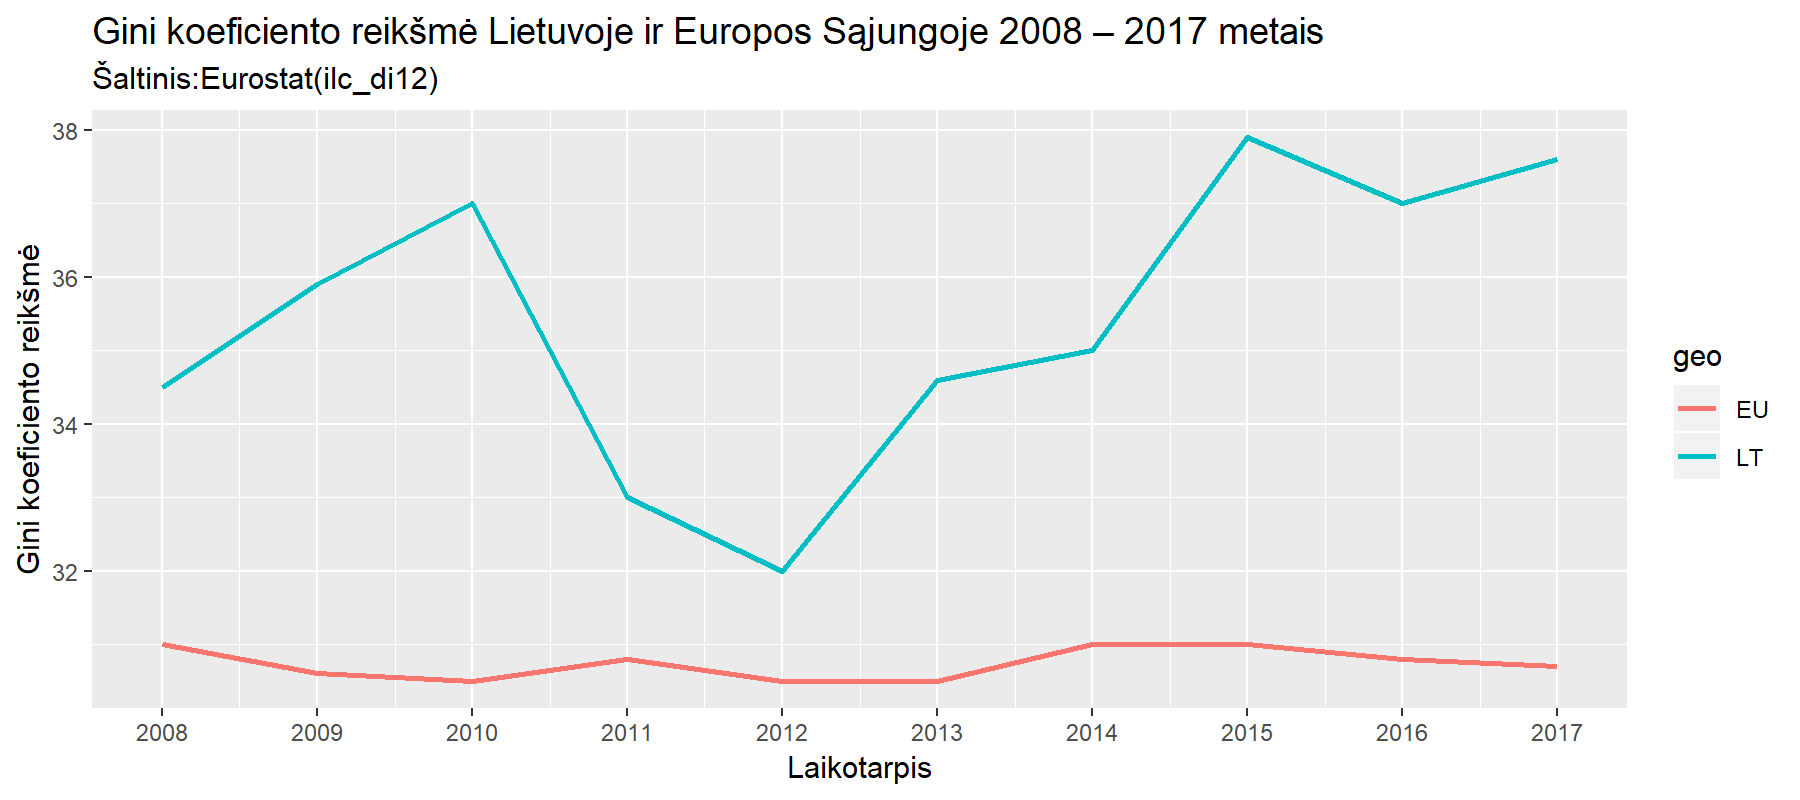
\includegraphics[scale=0.7]{LTginiFrom2008.png}
\caption{Gini koeficiento reikšmė Lietuvoje ir Europos Sąjungoje 2008 - 2017 metais}
\end{figure}
Kaip matome pagal 1 grafiką, Džini koeficientas Lietuvoje 2008 - 2017 metais svyravo nuo 32\% iki 37.9\%, palyginus su Europos Sąjungos vidurkiu, kuris svyravo nuo 30.5\% iki 31\%, Lietuvoje nelygybė buvo santykinai didelė, nes visada viršijo 30\% ir tik 2011 ir 2012 metais buvo priartėjus prie vidurkio(33\% ir 32\%), tačiau jo nepasiekė. Nuo 2012 iki 2015 metų koeficientas tik didėjo, 2016 buvo 0.9\% nukritęs, tačiau 2017 metais vėl pakilo.
\begin{figure}[H]
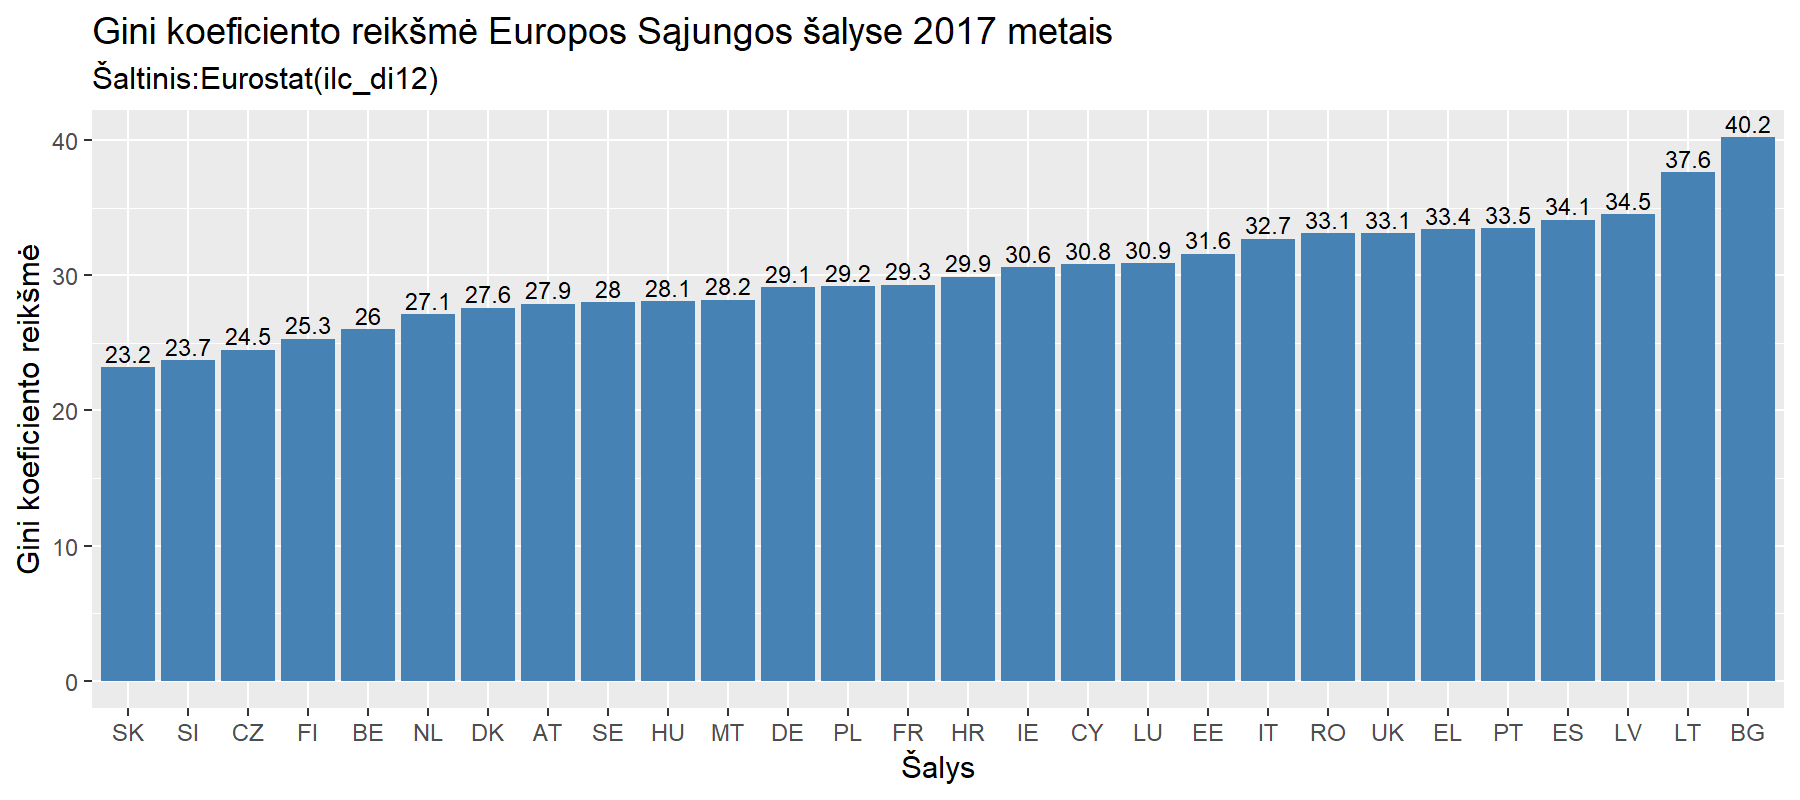
\includegraphics[scale=0.7]{AllGini2017.png}
\caption{Gini koeficiento reikšmė Europos Sąjungos šalyse 2017 metais}
\end{figure}
Pagal 2 grafiką matome, kad 2017 metais Gini koeficientas buvo lygus 37.6\% ir tarp visų Europos Sąjungos šalių, Lietuva buvo antroje vietoje pagal didumą. Tai reiškia, kad paskutiniais duomenimis, Lietuvoje pajamų nelygybė yra viena didžiausių ES ir yra net apie 1.6 karto didesnė negu Slovakijoje, kur pajamų nelygybė pagal labiausiai paplitusį pajamų nelygybės rodiklį yra mažiausia.
\subsection{Ranginiai matavimai}
Įprastinė statistika, operuojanti vidutiniais dydžiais, dažnai nepajėgi užfiksuoti už šių vidurkių besislepiančio didelio
atotrūkio tarp atskirų dydžių kraštutinių verčių. Tai atskleidžia
atskirų decilinių ar kvintilinių visuomenės grupių analizės. (\cite{lisauskaite2010lietuvos})
Decilinis pajamų pasiskirstymas yra vienas paprasčiausių pajamų nelygybės raiškos būdų. Deciliai gaunami į 10 lygių dalių padalijus gyventojus pagal jų pajamas didėjimo tvarka. Taip skirstant gaunama 10 grupių, iš kurių pirmoji, vadinama pirmuoju deciliu (D1), atitinka 10\% žmonių, gaunančių mažiausias vienam namų ūkio nariui pajamas per mėnesį, o dešimtasis decilis (D10) rodo 10\% turtingiausių gyventojų vidutines pajamas, tenkančias vienam namų ūkio nariui per mėnesį. Decilinis pajamų pasiskirstymas leidžia įvertinti gyventojų pajamų pasiskirstymo netolygumą, t. y. vargingiausių ir turtingiausių gyventojų grupių pajamų diferenciaciją. 
\begin{figure}[H]
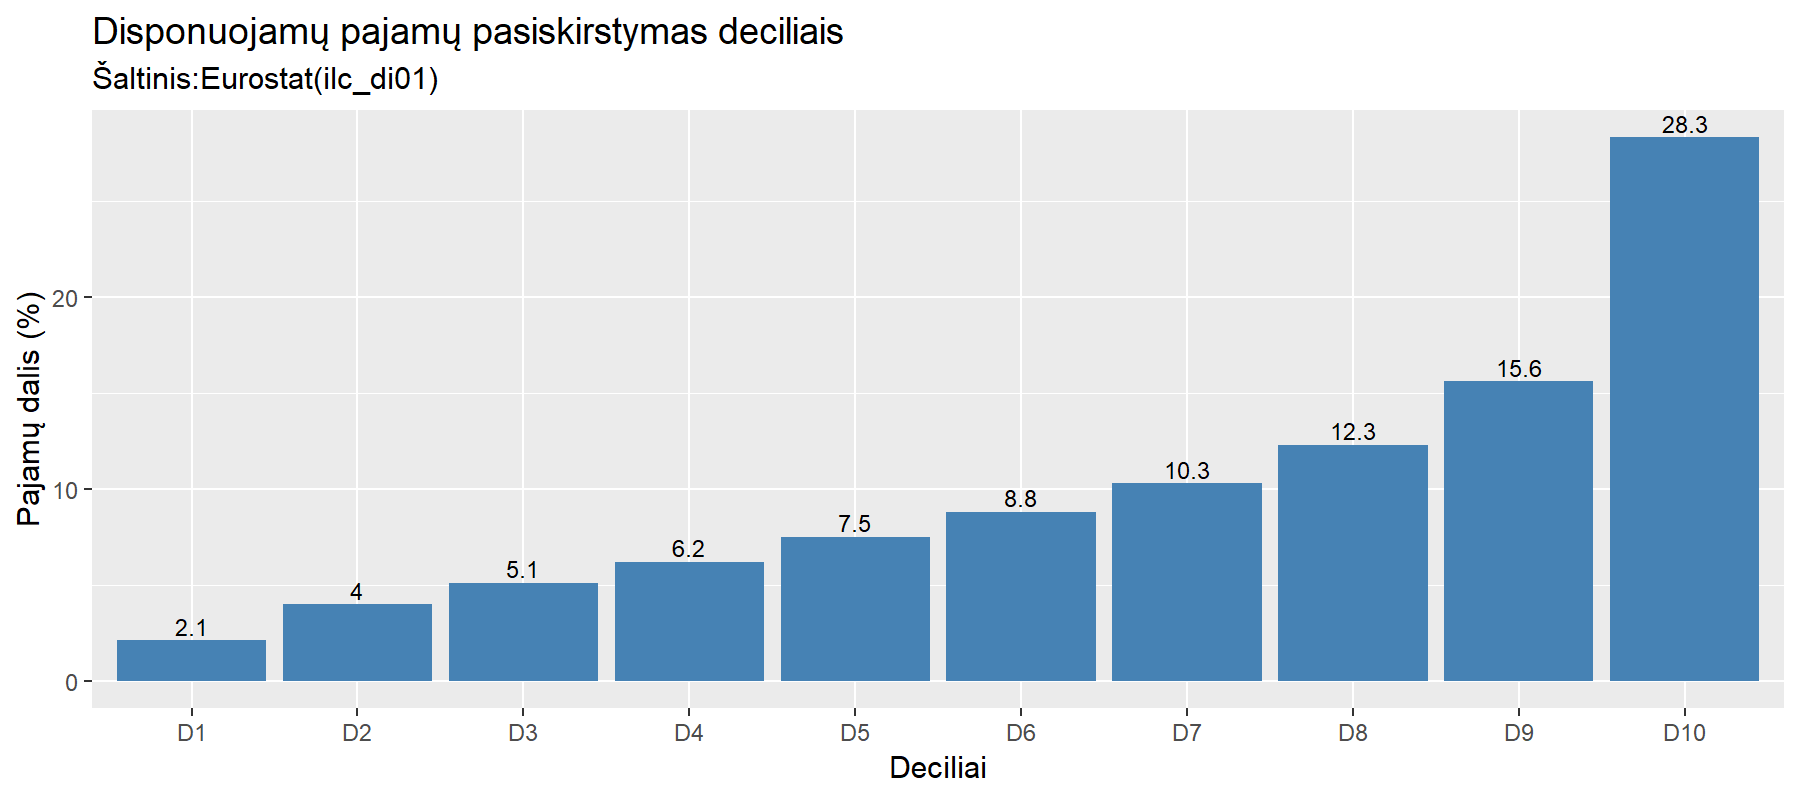
\includegraphics[scale=0.7]{LTdeciles2017.png}
\caption{Disponuojamų pajamų pasiskirstymas deciliais}
\end{figure}
Kaip matome pagal 3 grafiką, aštuoni vidutiniai pajamų deciliai tarpusavyje nelabai skiriasi. Pajamų dalies skirtumas tarp gretimų decilių svyruoja nuo 1.1\% iki 3.3\%. Tačiau ypač ryškus atotrūkis matomas tarp devinto ir dešimto decilių, kuris yra lygus net 12.7\%, o kraštutinių decilių išsiskiriančios pajamos turi didelę įtaką nelygybės rodikliams. Taip pat matome, kad turtingiausia gyventojų dalis (dešimtasis decilis) uždirba daugiau nei penkios skurdžiausos gyventojų grupės (pirmi penki deciliai) kartu sudėjus. Pajamų paskirstymo tarp askirų visuomenės dalių nelygybę labai vaizdžiai atskleidžia disponuojamų pajamų dalys pajamų deciliuose, parodančios, kokią visų gyventojų disponuojamų pajamų dalį sudaro atitinkamo decilio gyventojų pajamos.(\cite{lazutka2003gyventojku}) Kol skurdžiausias visuomenės 2017 metais turėjo pasitenkinti 2.1\% visų pajamų, tuo tarpu tokio pat dydžio turtingiausia visuomenės dalis disponavo 28.3\% visų pajamų.
\begin{figure}[H]
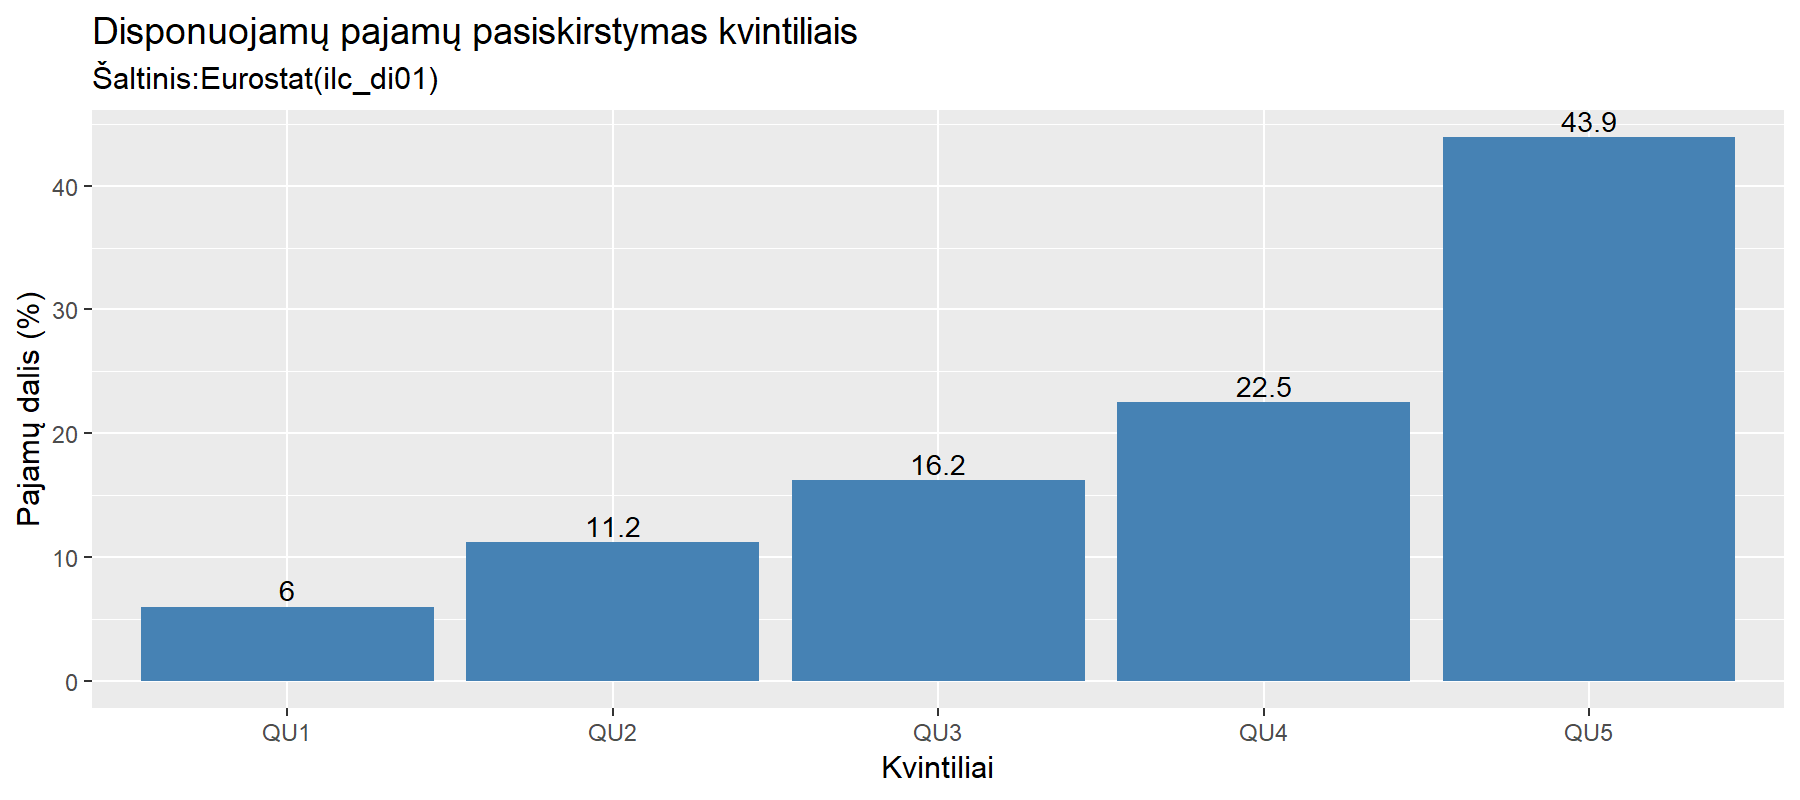
\includegraphics[scale=0.7]{LTquantiles2017.png}
\caption{Disponuojamų pajamų pasiskirstymas kvintiliais}
\end{figure}
Taip pat gali būti ir kvintilinis pajamų paskirstymas. Kvintiliai suskirsto gyventojų pajamų duomenų seką, išdėstytą didėjimo tvarka į penkias lygias dalis. Pirmasis Kvintilis (QU1) – parodo 20 proc. mažiausias pajamas gaunančių gyventojų vidutines pajamas. QU5 parodo 20 proc. turtingiausių gyventojų vidutines pajamas.\\
Kaip matyti iš 4 grafiko duomenų, 2017 metais Lietuvoje 20\% turtingiausių gyeventojų disponavo net 43.9\%, o 20\% skurdžiausių gyventojų tik 6\%.  \\
Pajamų nelygybei matuoti skaičiuojamas kvintilių diferenciacijos koeficientas, lygus  santykiui QU5/QU1 t.y. kraštinių kvintilių santykis, kuris parodo, kiek kartų 20 procentų turtingiausių gyventojų pajamos viršija 20 procentų skurdžiausių gyventojų pajamas. \\
\begin{table}[h!]
\centering
\begin{center}
 \begin{tabular}{ |p{3cm}||p{3cm}|p{3cm}|p{3cm}|  }
 \hline
 \multicolumn{2}{|c|}{Kraštinių kvantilių santykis Lietuvoje} \\
 \hline
 Metai & Vertė\\
 \hline
2017 & 7.3 \\
2016 & 7.1 \\
2015 & 7.5 \\ 
2014 & 6.1 \\
2013 & 6.1 \\
2012 & 5.3 \\
2011 & 5.8 \\
2010 & 7.3 \\
2009 & 6.4 \\
2008 & 6.1 \\
 \hline
\end{tabular}
\end{center}
\caption{Šaltinis:Eurostat ($ilc di11$)}
\label{table:1}
\end{table}
Kaip matome pagal 1 lentelės duomenis, Lietuvoje nuo 2008 metų 20\% turtingiausių gyventojų disponavo bent šešiais kartais daugiau pajamų negu 20\% procent skurdžiausių Lietuvos gyventojų, o per paskutinius trejus metus  net daugiau nei septynis kartus.
\section{Pajamų nelygybė ir kiti rodikliai}
\subsection{Pajamų nelygybė ir skurdas}
Pagal Europos Komisiją, nelygybė lemia padidėjęs skurdas žemiausiame pajamų pasiskirstymo segmente. Jei mažiausias pajamas gaunantys (arba mažiausiai turto turintys) asmenys stokoja lėšų, kad galėtų investuoti į savo įgūdžius ir išsimokslinimą, gali būti, kad jie negalės išnaudoti visų galimybių, o tai daro žalą visos ekonomikos augimui. Be to, pajamų perskirstymas taip pat gali padėti skatinti paklausos šalies ekonomikoje augimą, nes mažas pajamas gaunantys namų ūkiai linkę išleisti daugiau.
\begin{figure}[H]
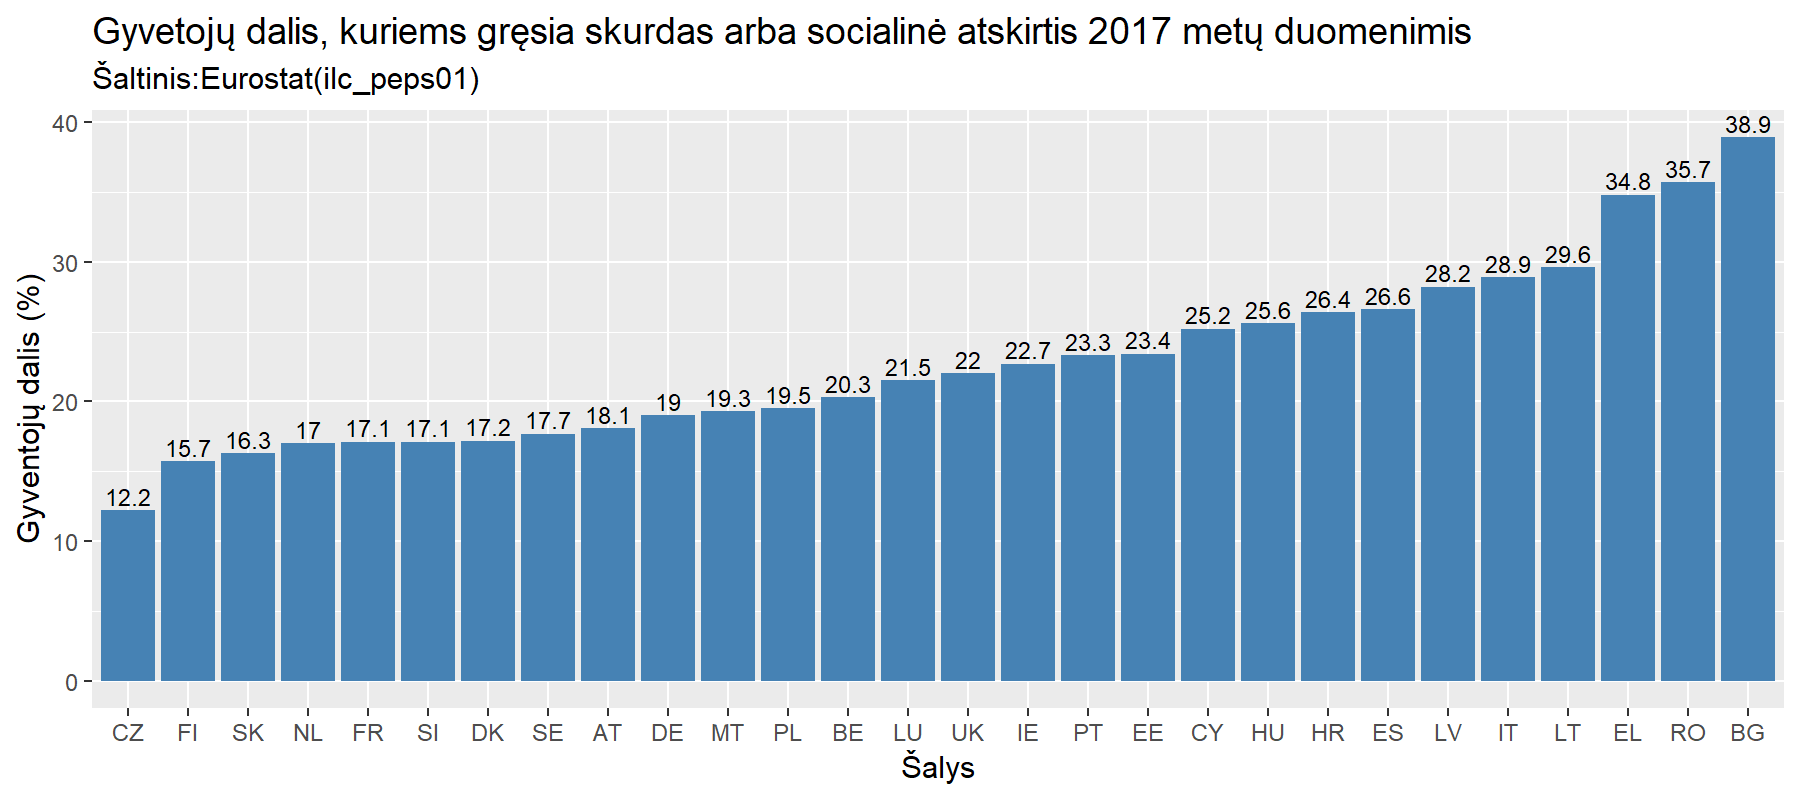
\includegraphics[scale=0.7]{povertyrisk.png}
\caption{Gyvetojų dalis, kuriems gręsia skurdas arba socialinė atskirtis 2017 metų duomenimis}
\end{figure}
Kaip matome pagal 5 grafiką, tais pačiais metais, kai Lietuva pagal pajamų nelygybę tarp visų Europos Sąjungos šalių buvo antroje vietoje, net 29.6\% gyventojų buvo socialinės atskirties ir skurdo rizikoje, tai, už šį rezultatą aukšiau buvo tik trys Europos Sąjungos šalys. Taigi, iš to galima spręsti kad šie du rodikliai yra glaudžiai susiję.
\subsection{Pajamų nelygybė ir sveikata}
Gyventojų sveikatos ir kitos socialinės problemos atsiranda ne tiek dėl jų gaunamų mažų pajamų, kiek dėl visuomenėje egzistuojančios gyventojų pajamų nelygybės ir to, kaip pats žmogus save vertina kitų atžvilgiu. Jei žmogus mano, kad jo socialinis statusas visuomenėje yra žemas, jis nebus nei laimingas, nei optimistiškai
nusiteikęs. Pastovi kova už didesnes pajamas ir aukštesnį socialinį statusą visuomenėje, ypač laisvosios rinkos ekonomikos modelius diegiančiose ir didelę ekonominę nelygybę turinčiose šalyse, sukuria pastovią stresinę aplinką. To padariniai – prastėjanti žmonių sveikata, augantis nusikalstamumas ir kitos socialinės problemos. (\cite{buivydas2011ar})
Siekiant įvertinti, kokią įtaką nelygybė galėtų turėti Lietuvos gyventojų sveikatai, Buivydas ir Černiauskas ieškojo ryšio tarp namų ūkių išlaidų nelygybės ir vidutinės tikėtinos gyvenimo trukmės bei mirtingumo rodiklių, ir ryšį pamatė esantį labai stiprų. Jie teigė, kad galimai šalies gyventojai, mūsų visuomenėje besikaupiantį stresą dėl socialinės–ekonominės nelygybės išreiškia ne tik per labai žemą pasitikėjimą vykdomosios ir atstovaujamosios valdžios
institucijomis, bet ir bandydami pamiršti tas problemas vartojant alkoholį.
\subsection{Pajamų nelygybė ir nusikalstamumas}
Smurtinių nusikaltimų nelygybės poveikis yra didelis. Nors dauguma nusikaltimų yra daromi labiausiai socialiai nukentėjusių visuomenės narių, šitie asmenys patiria didesnį spaudimą ir paskatas juos daryti ten, kur yra didesnė pajamų nelygybė.(\cite{kelly2000inequality}) Globaliajame kontekste galima pastebėti tendenciją, kad pajamų
nelygybė yra tiesiogiai siejama su nužudymų didėjimo tempais. Šis ryšys ypač stiprus, kai persidengia su ekonomine diskriminacija dėl rasės, religijos ar etninių grupių. (\cite{skuvciene2008pajamku})
\subsection{Pajamų nelygybė ir vartojimas}
V. Lisauskaitės skaičiavimais, Lietuvos gyventojų vartojimo
išlaidų dydžiai kraštutiniuose deciliuose 2008-2010 metais
skyrėsi net apie 8 kartus. Ypač dideli skirtumai – poilsio ir kultūros, būsto apstatymo, drabužių ir avalynės įsigijimo srityse.
Gyventojai, patenkantys į pirmuosius du decilius, didžiąją
dalį pajamų sunaudoja einamajam vartojimui ir būtiniausioms reikmėms, mažiausiai dėmesio gali skirti poilsiui ir
kultūrai, švietimui, sveikatos priežiūrai - veiksniams, nuo
kurių labiausiai priklauso žmogaus gyvenimo kokybė. Ryškūs vartojimo išlaidų skirtumai tarp gretimų decilių, kai kuriose išlaidų grupėse siekiantys du ir net tris kartus, liudija ryškią turtinę diferenciaciją ir pasiturinčios visuomenės mažumos egzistavimą, tuo pačiu metu penktadaliui Lietuvos gyventojų balansuojant ties skurdo riba. (\cite{lisauskaite2010lietuvos})
\section{Išvados}
Pajamų nelygybė suprantama kaip pajamų skirtumai tarp tam tikrų visuomenės grupių. Kaip jau sužinojome, individai gali būti suskirstyti pagal uždirbamas pajamas į penkias arba dešimt dalių, tos dalys atitinkamai vadinsis kvintiliai ir deciliai. Pagal kraštinių decilių arba kvintilių santykį galima spręsti apie pajamų nelygybės dydį. Kaip matėme pagal 2008 – 2017 metų duomenis, Lietuvoje penktadalis turtingiausių gyventojų disponavo bent šešiais kartais daugiau pajamų negu penktadalis vargingiausiai gyvenančių žmonių. Taip pat apie pajamų pajamų galima spręsti pagal Džini koeaficientą. Lietuvoje Džini koeficientas 2008 – 2017 metais nuo vieno iki septynių procentų viršijo Europos Sąjungos vidurkį. Pajamų nelygybė Lietuvoje tebėra viena didžiausių Europos Sąjungoje ir todėl reiktų kuo daugiau skirti jai dėmesio, nes ji taip pat yra glaudžiai susijusi ir su padidėjusiu nusikalstamumu ir mirtingumo rodikliais, suprastėjusia sveikata, vartojimo diferenciacija.

\newpage
\nocite{*}
\printbibliography[title={Literatūra}]
\end{document}